%%%%%%%%%%%%%%%%%%%%%%%%%%%%%%%%%
%%%%%%% Dokumentdefinition %%%%%%
%%%%%%%%%%%%%%%%%%%%%%%%%%%%%%%%%
\documentclass[oneside,12pt,a4paper,bibliography=totoc,numbers=noenddot,table]{scrreprt} % scrreprt
\usepackage{geometry}
\geometry{a4paper,top=30mm, left=30mm, right=30mm, bottom=30mm, headsep=5mm, footskip=10mm}
\setlength{\footheight}{20.77846pt}
\setlength{\headheight}{20.77846pt}

\usepackage{setspace} % Zeilenabstand

%%%%%%%%%%%%%%%%%%%%%%%%%%%%%%%
%Kopf- und Fußzeilendefinition%
%%%%%%%%%%%%%%%%%%%%%%%%%%%%%%%
\usepackage[headsepline,footsepline]{scrlayer-scrpage} % mit Trennlinien

\pagestyle{scrheadings} % Seitenstil umdefiniert
\clearscrheadfoot % Definition leermachen
\renewcommand{\chapterpagestyle}{scrheadings}		%Kapitelseitenstil umdefiniert
\renewcommand{\chaptermark}[1]{\markboth{\ #1}{}}	%Definition Kapitel?berschrift=\leftmark
\ohead{\sffamily\upshape\leftmark} % äußere Kopfzeile
%\chead{} % mittlere Kopfzeile
\ihead{}  % innere Kopfzeile
\ofoot{\sffamily\upshape\thepage} % äußere Fu?zeile
%\cfoot{\upshape\thepage} % mittlere Fu?zeile
\ifoot{} % innere Fußzeile

%%%%%%%%%%%%%%%%%%%%%%%%%%%%%%%%%%%%%%%
%%%%%%%deutsche Zeichenkodierung%%%%%%%
%%%%%%%%%%%%%%%%%%%%%%%%%%%%%%%%%%%%%%%
%\usepackage[utf8]{inputenc}
\usepackage[english,ngerman]{babel}
%%%%%%%%%%%%%%%%%%%%%%%%%%%%%%%%%%%%%%%%%%%%%%
%%%%%%%%%%%%Verschiedene Schriftarten%%%%%%%%%
%%%%%%%%%%%%%%%%%%%%%%%%%%%%%%%%%%%%%%%%%%%%%%
%\usepackage{kpfonts}
%\usepackage{stix} % this was selected by default
%\usepackage{times}
%\usepackage{libertinust1math}
%\usepackage[T1]{fontenc}
\usepackage{amsmath,amssymb,unicode-math}

%\renewcommand*\familydefault{\sfdefault}

%\usepackage[sfdefault]{roboto}  %% Option 'sfdefault' only if the base font of the

  \setmainfont{Source Serif Pro}

  \setsansfont{Source Sans Pro}

  \setmonofont[Mapping=tex-ansi,Scale=0.75]{Source Code Pro}

  %\setmathfont{Latin Modern Math}

%%%%%%%%%%%%%%%%%%%%%%%%%%%%%%%%%%%%%%%%%%%%%%
%%%%%%%%%%%%%%%Zusatzpackages%%%%%%%%%%%%%%%%%
%%%%%%%%%%%%%%%%%%%%%%%%%%%%%%%%%%%%%%%%%%%%%%
\usepackage{a4wide}
%\usepackage[locale=DE]{siunitx}
\usepackage{acronym}					%Abk?rzungsverzeichnis
\usepackage[nointegrals]{wasysym}		%Symbole und Sonderzeichen
\usepackage{romannum}					%R?mische Zahlen
%\usepackage{floatflt,epsfig} 			%Bilder im eps-format einf?gen
\usepackage{graphicx}
\usepackage[hyphens]{url}				%Websites einbinden
\usepackage{pdfpages} 					%direkt pdf Datein einbinden
\usepackage{mathtools}					%matheumgebung f?r Formeln und Gleichungen
\usepackage{capt-of}					%Captions f?r non-float-Objekte
\usepackage[titletoc]{appendix}			%erm?glicht das erstellen von Anhangsverzeichnissen
% Typography
\usepackage{microtype}                  % Typographievoodoo
\usepackage{csquotes}
\usepackage[all]{nowidow}
%\clubpenalty = 10000
%\widowpenalty = 10000

%%%%%%%%%%%%%%%%%%%%%%%%%%%%%%%%%%%%%%%%%%%%%%%%%%%%%%%%%%%%%%
% Extra stuff for Rmarkdown to work (code blocks)
%%%%%%%%%%%%%%%%%%%%%%%%%%%%%%%%%%%%%%%%%%%%%%%%%%%%%%%%%%%%%%
\providecommand{\tightlist}{%
  \setlength{\itemsep}{0pt}\setlength{\parskip}{0pt}}
\usepackage{framed}
\definecolor{shadecolor}{RGB}{248,248,248}
\newenvironment{Shaded}{\begin{snugshade}}{\end{snugshade}}
\usepackage{fancyvrb}
\newcommand{\VerbBar}{|}
\newcommand{\VERB}{\Verb[commandchars=\\\{\}]}
\DefineVerbatimEnvironment{verbatim}{Verbatim}{xleftmargin=0em}
\DefineVerbatimEnvironment{Highlighting}{Verbatim}{xleftmargin=0em,commandchars=\\\{\}}

\newcommand{\KeywordTok}[1]{\textcolor[rgb]{0.13,0.29,0.53}{\textbf{{#1}}}}
\newcommand{\DataTypeTok}[1]{\textcolor[rgb]{0.13,0.29,0.53}{{#1}}}
\newcommand{\DecValTok}[1]{\textcolor[rgb]{0.00,0.00,0.81}{{#1}}}
\newcommand{\BaseNTok}[1]{\textcolor[rgb]{0.00,0.00,0.81}{{#1}}}
\newcommand{\FloatTok}[1]{\textcolor[rgb]{0.00,0.00,0.81}{{#1}}}
\newcommand{\ConstantTok}[1]{\textcolor[rgb]{0.00,0.00,0.00}{{#1}}}
\newcommand{\CharTok}[1]{\textcolor[rgb]{0.31,0.60,0.02}{{#1}}}
\newcommand{\SpecialCharTok}[1]{\textcolor[rgb]{0.00,0.00,0.00}{{#1}}}
\newcommand{\StringTok}[1]{\textcolor[rgb]{0.31,0.60,0.02}{{#1}}}
\newcommand{\VerbatimStringTok}[1]{\textcolor[rgb]{0.31,0.60,0.02}{{#1}}}
\newcommand{\SpecialStringTok}[1]{\textcolor[rgb]{0.31,0.60,0.02}{{#1}}}
\newcommand{\ImportTok}[1]{{#1}}
\newcommand{\CommentTok}[1]{\textcolor[rgb]{0.56,0.35,0.01}{\textit{{#1}}}}
\newcommand{\DocumentationTok}[1]{\textcolor[rgb]{0.56,0.35,0.01}{\textbf{\textit{{#1}}}}}
\newcommand{\AnnotationTok}[1]{\textcolor[rgb]{0.56,0.35,0.01}{\textbf{\textit{{#1}}}}}
\newcommand{\CommentVarTok}[1]{\textcolor[rgb]{0.56,0.35,0.01}{\textbf{\textit{{#1}}}}}
\newcommand{\OtherTok}[1]{\textcolor[rgb]{0.56,0.35,0.01}{{#1}}}
\newcommand{\FunctionTok}[1]{\textcolor[rgb]{0.00,0.00,0.00}{{#1}}}
\newcommand{\VariableTok}[1]{\textcolor[rgb]{0.00,0.00,0.00}{{#1}}}
\newcommand{\ControlFlowTok}[1]{\textcolor[rgb]{0.13,0.29,0.53}{\textbf{{#1}}}}
\newcommand{\OperatorTok}[1]{\textcolor[rgb]{0.81,0.36,0.00}{\textbf{{#1}}}}
\newcommand{\BuiltInTok}[1]{{#1}}
\newcommand{\ExtensionTok}[1]{{#1}}
\newcommand{\PreprocessorTok}[1]{\textcolor[rgb]{0.56,0.35,0.01}{\textit{{#1}}}}
\newcommand{\AttributeTok}[1]{\textcolor[rgb]{0.77,0.63,0.00}{{#1}}}
\newcommand{\RegionMarkerTok}[1]{{#1}}
\newcommand{\InformationTok}[1]{\textcolor[rgb]{0.56,0.35,0.01}{\textbf{\textit{{#1}}}}}
\newcommand{\WarningTok}[1]{\textcolor[rgb]{0.56,0.35,0.01}{\textbf{\textit{{#1}}}}}
\newcommand{\AlertTok}[1]{\textcolor[rgb]{0.94,0.16,0.16}{{#1}}}
\newcommand{\ErrorTok}[1]{\textcolor[rgb]{0.64,0.00,0.00}{\textbf{{#1}}}}
\newcommand{\NormalTok}[1]{{#1}}

%%%%%%%%%%%%%%%%%%%%%%%%%%
%%%%% kableExtra stuff
%%%%%%%%%%%%%%%%%%%%%%%%%%
\usepackage{booktabs}
\usepackage{longtable}
\usepackage{array}
\usepackage{multirow}
\usepackage{xcolor}
\usepackage{wrapfig}
\usepackage{float}
\usepackage{colortbl}
\usepackage{pdflscape}
\usepackage{tabu}
\usepackage{threeparttable}
\usepackage{threeparttablex}
\usepackage[normalem]{ulem}
\usepackage{makecell}

%\usepackage{natbib}

%%%%%%%%%%%%%%%%%%%%%%%%%%%%%%%%%%%%%%%%
%%% Stil des Literaturverzeichnisses %%%
%%%%%%%%%%%%%%%%%%%%%%%%%%%%%%%%%%%%%%%%

\usepackage[
    backend=biber,
    natbib=true,
    style=apa,
    %bibstyle=authoryear, citestyle=apa,
    %style=authoryear,
    sorting=nyt,
    %sortlocale=de_DE,
    sortlocale=en_US,
    url=false,
    doi=true,
]{biblatex}

\setlength\bibitemsep{1.5\itemsep}

\addbibresource{references.bib}

\DeclareLanguageMapping{ngerman}{ngerman-apa}
\DeclareLanguageMapping{english}{english-apa}
\AtBeginDocument{\selectlanguage{ngerman}\selectlanguage{english}}

%%%%%%%%%%%%%%%%%%%%%%%%%%%%%%%%%%%%%%%%%%%
%%%%%%%%%%%%%% Special Stuff %%%%%%%%%%%%%%
%%%%%%%%%%%%%%%%%%%%%%%%%%%%%%%%%%%%%%%%%%%
\usepackage[colorlinks,    				%PDF linked Verzeichnis
pdfpagelabels,
pdfstartview = FitH,
bookmarksopen = true,
bookmarksnumbered = true,
linkcolor = black,
plainpages = false,
hypertexnames = false,
citecolor = black,
breaklinks = true,
allcolors = black] {hyperref}

%\renewcommand{\labelitemi}{-}   %aufzählungszeichen strich statt punkt - beliebig anpassbar

% \sloppy % "schlampiger" Blocksatz

% Absatzeinzug und Abstand
% \setlength{\parindent}{0.5cm}
\setlength{\parindent}{0cm}
% \setlength{\parskip}{0.1cm}

%%%%%%%%%%%%%%%%%%%%%%%%%%%%%%%%%%%%%%%
% hier startet das eigentliche Dokument
%%%%%%%%%%%%%%%%%%%%%%%%%%%%%%%%%%%%%%%
\begin{document}
\pagenumbering{Roman}				% Seitennummerierung auf römisch geändert

%%%%%%%%%%%%%%%%%%%%%%%%%%%%%%%%%%%%%%%%%%%
% Deckblatt
%%%%%%%%%%%%%%%%%%%%%%%%%%%%%%%%%%%%%%%%%%%
\begin{titlepage}
\thispagestyle{empty}
\begin{center}

%\begin{LARGE}
\textsf{\textbf{Faculty 9824}}\\
%\end{LARGE}

\begin{figure}[h!]
    \centering
    
\includegraphics[height=2cm]{includes/UniBremen.pdf}
\end{figure}

\textsf{\textbf{Institute name}}\\[1,0cm]

\begin{Large}
    \textsf{\textbf{Master Thesis}}\\[0,75cm]
\end{Large}

\begin{LARGE}
    \textsf{\textbf{Thesis Title}}\\[1,5cm]
\end{LARGE}

%\vspace{1.5em}

\vfill

\begin{large}
    \textsf{by}\\[0,1cm]
    \textsf{\textbf{Your Name}}\\[0,1cm]
    \textsf{born Date in Birthplace}\\[0,1cm]
    \textsf{Matr.-Nr.: 3482423}\\

    \vspace{0.5em}

    \textsf{2020-04-25}
\end{large}

\vfill

\begin{large}
    \textsf{\textbf{Supervisors:}}\\[0,3cm]
        \textsf{Supervisor 1}\\[0.5em]
        \textsf{Supervisor 2}\\[0.5em]
    \end{large}

\end{center}

\end{titlepage}
\thispagestyle{empty}
\cleardoublepage

\newpage

%%%%%%%%%%%%%%%%%%%%%%%%%%%%%%%%%%%%%%%%%%%
%%%%%%%%%%%%%%% Verzeichnisse %%%%%%%%%%%%%
%%%%%%%%%%%%%%%%%%%%%%%%%%%%%%%%%%%%%%%%%%%
\setcounter{secnumdepth}{2} 	%countertiefe für Verzeichnisse
\setcounter{page}{1}

\chaptermark{Table of Contents}
\tableofcontents
\newpage



%%%%%%%%%%%%%%%%%%%%%%%%%%%%%%%%%%%%%%%%%%%
%%%%%%%%%%%%%%% Main text %%%%%%%%%%%%%%%%%
%%%%%%%%%%%%%%%%%%%%%%%%%%%%%%%%%%%%%%%%%%%
% Not needed <here>, but has to be included in Rmd before main content
% \setcounter{page}{1}

% Hopefully working linespread comparable to word
%\linespread{1.25}
%\setstretch{1.433}
% \linespread{1.3}
\onehalfspacing
\setlength{\parskip}{0.25cm}

%\onehalfspacing

\hypertarget{abstract}{%
\chapter*{Abstract}\label{abstract}}
\addcontentsline{toc}{chapter}{Abstract}

\chaptermark{Abstract}

The abstract should outline the main approach and findings of the thesis and must not be more than 500 words.

\newpage

\clearpage\pagenumbering{arabic}\setcounter{page}{1}

\hypertarget{ch:intro}{%
\chapter{Introduction}\label{ch:intro}}

This is where you introduce the main ideas of your thesis, and an overview of the context and background.

In a PhD, Chapter 2 would normally contain a literature review. Typically, Chapters 3--5 would contain your own contributions. Think of each of these as potential papers to be submitted to journals. Finally, Chapter 6 provides some concluding remarks, discussion, ideas for future research, and so on. Appendixes can contain additional material that don't fit into any chapters, but that you want to put on record. For example, additional tables, output, etc.

\hypertarget{rmarkdown}{%
\section{Rmarkdown}\label{rmarkdown}}

In this template, the rest of the chapter shows how to use Rmarkdown. The big advantage of using Rmarkdown is that it allows you to include your R code directly into your thesis, to ensure there are no errors in copying and pasting, and that everything is reproducible. It also helps you stay better organized.

For details on using \emph{R Markdown} see \url{http://rmarkdown.rstudio.com}.

\hypertarget{results-from-analyses}{%
\section{Results from analyses}\label{results-from-analyses}}

We can fit a dynamic regression model to the sales data.

If \(y_t\) denotes the sales in quarter \(t\), \(x_t\) denotes the corresponding advertising budget and \(z_t\) denotes the GDP, then the resulting model is:
\begin{equation}
  y_t - y_{t-4} = \beta (x_t-x_{t-4}) + \gamma (z_t-z_{t-4}) + \theta_1 \varepsilon_{t-1} + \Theta_1 \varepsilon_{t-4} + \varepsilon_t
\end{equation}
where

The \texttt{knitLatex} package is useful for generating tables from R output. Other packages can do similar things including the \texttt{kable} function in \texttt{knitr} which is somewhat simpler but you have less control over the result. If you use \texttt{knitLatex} to generate tables, don't forget to include \texttt{results="asis"} in the chunk settings.

\hypertarget{unrelated-code}{%
\section{Unrelated Code}\label{unrelated-code}}

A plot

\begin{Shaded}
\begin{Highlighting}[]
\KeywordTok{library}\NormalTok{(ggplot2)}
\KeywordTok{library}\NormalTok{(hrbrthemes)}
\end{Highlighting}
\end{Shaded}

\begin{verbatim}
## NOTE: Either Arial Narrow or Roboto Condensed fonts are required to use these themes.
\end{verbatim}

\begin{verbatim}
##       Please use hrbrthemes::import_roboto_condensed() to install Roboto Condensed and
\end{verbatim}

\begin{verbatim}
##       if Arial Narrow is not on your system, please see https://bit.ly/arialnarrow
\end{verbatim}

\begin{Shaded}
\begin{Highlighting}[]
\KeywordTok{ggplot}\NormalTok{(iris, }\KeywordTok{aes}\NormalTok{(}\DataTypeTok{x =}\NormalTok{ Sepal.Length, }\DataTypeTok{y =}\NormalTok{ Sepal.Width, }\DataTypeTok{fill =}\NormalTok{ Species)) }\OperatorTok{+}
\StringTok{  }\KeywordTok{geom\_point}\NormalTok{(}\DataTypeTok{shape =} \DecValTok{21}\NormalTok{, }\DataTypeTok{size =} \DecValTok{2}\NormalTok{) }\OperatorTok{+}
\StringTok{  }\KeywordTok{theme\_ipsum}\NormalTok{(}
    \DataTypeTok{base\_family =} \StringTok{"Source Sans Pro"}
\NormalTok{  )}
\end{Highlighting}
\end{Shaded}

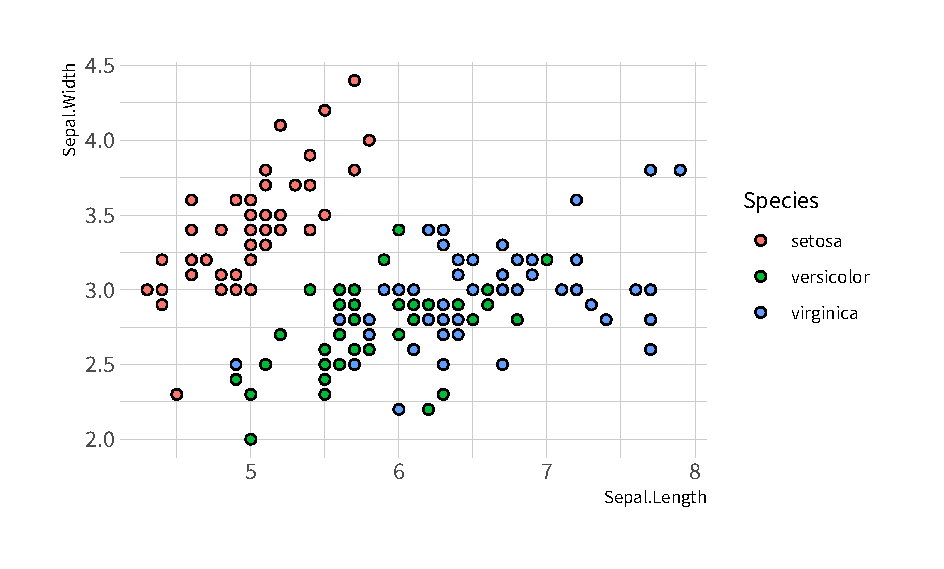
\includegraphics{thesis_files/figure-latex/a-plot-1.pdf}

A table

\begin{table}[H]
\centering
\begin{tabular}{rrrrl}
\toprule
Sepal.Length & Sepal.Width & Petal.Length & Petal.Width & Species\\
\midrule
5.1 & 3.5 & 1.4 & 0.2 & setosa\\
4.9 & 3.0 & 1.4 & 0.2 & setosa\\
4.7 & 3.2 & 1.3 & 0.2 & setosa\\
4.6 & 3.1 & 1.5 & 0.2 & setosa\\
5.0 & 3.6 & 1.4 & 0.2 & setosa\\
\addlinespace
5.4 & 3.9 & 1.7 & 0.4 & setosa\\
\bottomrule
\end{tabular}
\end{table}

\hypertarget{ch:litreview}{%
\chapter{Literature Review}\label{ch:litreview}}

This chapter contains a summary of the context in which your research is set.

Imagine you are writing for your fellow PhD students. Topics that are well-known to them do not have to be included here. But things that they may not know about should be included.

Resist the temptation to discuss everything you've read in the last few years. And you are not writing a textbook either. This chapter is meant to provide the background necessary to understand the material in subsequent chapters. Stick to that.

You will need to organize the literature review around themes, and within each theme provide a story explaining the development of ideas to date. In each theme, you should get to the point where your ideas will fit in. But leave your ideas to later chapters. This way it is clear what has been done beforehand, and what new contributions you are making to the research field.

All citations should be done using markdown notation as shown below. This way, your bibliography will be compiled automatically and correctly.

\hypertarget{sec:expsmooth}{%
\section{Exponential smoothing}\label{sec:expsmooth}}

Exponential smoothing was originally developed in the late 1950s. Because of their computational simplicity and interpretability, they became widely used in practice.

Empirical studies by \textcite{MH79} and \textcite{Metal82} found little difference in forecast accuracy between exponential smoothing and ARIMA models. This made the family of exponential smoothing procedures an attractive proposition .

The methods were less popular in academic circles until \textcite{OKS97} introduced a state space formulation of some of the methods, which was extended in \textcite{HKSG02} to cover the full range of exponential smoothing methods.

\hypertarget{appendix-appendix}{%
\appendix}


\hypertarget{additional-stuff}{%
\chapter{Additional Stuff}\label{additional-stuff}}

You might put some computer output here, or maybe additional tables.

Note that line 5 must appear before your first appendix. But other appendices can just start like any other chapter.

%\addcontentsline{toc}{chapter}{Bibliography}
%\chaptermark{Bibliography}
\singlespacing

%%%%%%%%%%%%%%%%%%
%% Bibliography %%
%%%%%%%%%%%%%%%%%%

% Okay so usually this should print the bibligraphy and add it to the TOC according
% to both stackoverflow people and the actual biblatex documentation (re: KOMA classes)
% \printbibliography[heading=bibintoc]
% But because I don't understand *something* and this doesn't actually work,
% I'll work around this like so:

% Manually print bib heading *only*
\printbibheading
% Then print the bibliography without heading
\printbibliography[heading=none]

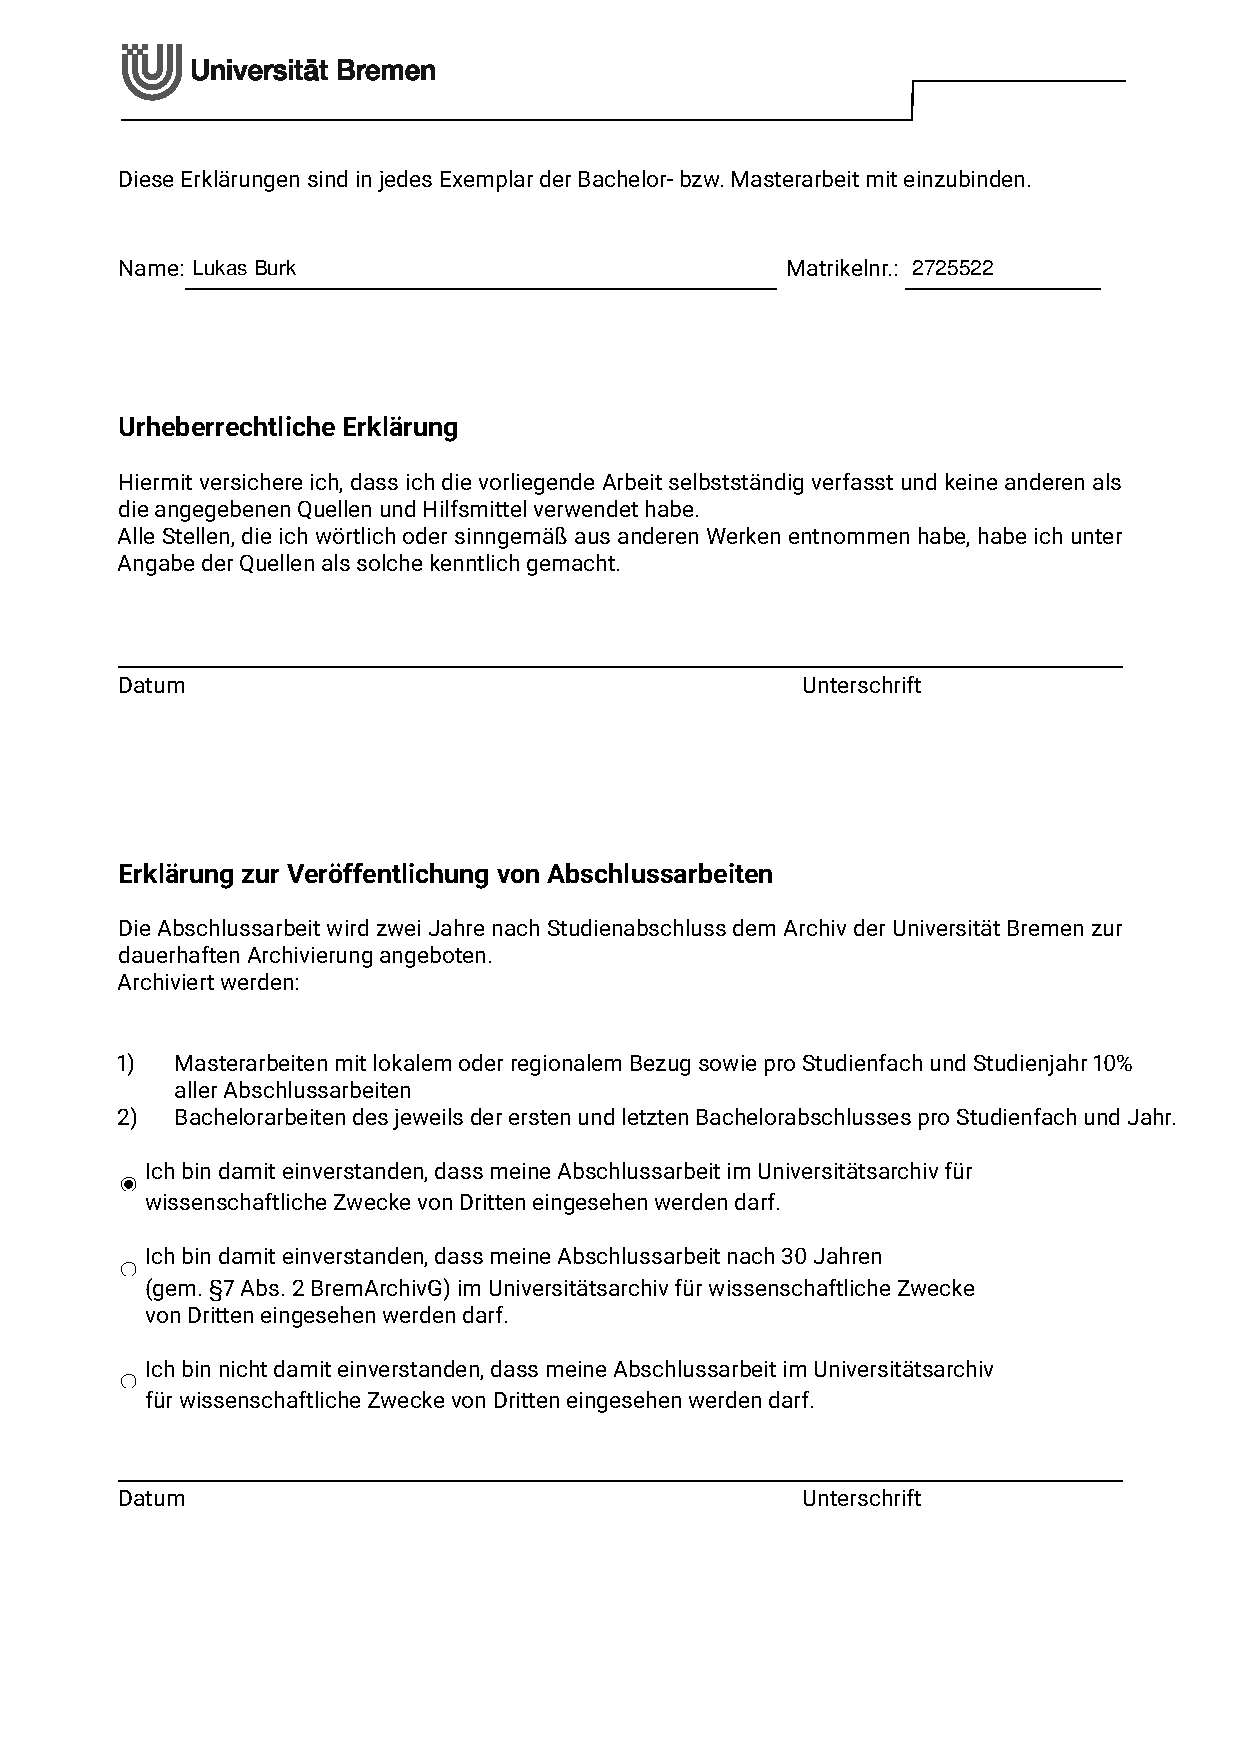
\includepdf[pages=1]{includes/erklaerung.pdf}

\end{document}
